\documentclass[11pt,a4paper]{article}
\usepackage[utf8]{inputenc}
\usepackage[spanish]{babel}
\usepackage{amsmath}
\usepackage{graphicx}
\usepackage{geometry}
\geometry{top=2.5cm, bottom=2.5cm, left=2.5cm, right=2.5cm}
\usepackage{fancyhdr}
\usepackage{xcolor}
\usepackage{hyperref}
\usepackage{booktabs}
\usepackage{titlesec}
\usepackage{caption}

% Colores institucionales
\definecolor{bankblue}{RGB}{20, 40, 80}
\definecolor{bankgold}{RGB}{240, 192, 64}
\definecolor{darkgray}{RGB}{74, 90, 114}

% Estilo de links
\hypersetup{
    colorlinks=true,
    linkcolor=bankblue,
    filecolor=magenta,      
    urlcolor=bankgold,
}

% Formato de títulos
\titleformat{\section}{\color{bankblue}\Large\bfseries}{\thesection}{1em}{}[\titlerule]
\titleformat{\subsection}{\color{darkgray}\large\bfseries}{\thesubsection}{1em}{}

% Encabezado y Pie
\pagestyle{fancy}
\fancyhf{}
\rhead{\textcolor{bankblue}{\textbf{Global Markets Research}}}
\lhead{Quantitative Risk Engine - BVL}
\cfoot{\thepage}

\begin{document}

\begin{titlepage}
    \centering
    \vspace*{4cm}
    
    {\Huge \textcolor{bankblue}{\textbf{Quantitative Risk Engine}} \par}
    \vspace{0.5cm}
    {\Large \textbf{Bolsa de Valores de Lima (BVL)} \par}
    
    \vspace{2cm}
    {\Large \textcolor{darkgray}{Reporte Metodológico de Optimización de Portafolios y Control de Riesgos} \par}
    
    \vspace{4cm}
    \textbf{Preparado por:}\\
    Quantitative Analytics Group\\
    \vspace{0.5cm}
    \today
    \vfill
    
    \begin{flushleft}
    \small \textit{Clasificación: CONFIDENCIAL / USO INTERNO}
    \end{flushleft}
\end{titlepage}

\tableofcontents
\newpage

\section{Resumen Ejecutivo}
El presente informe detalla el desarrollo e implementación de un \textbf{Motor Cuantitativo de Riesgo} diseñado para construir y auditar portafolios de inversión compuestos por activos de la Bolsa de Valores de Lima (BVL). 

Dada la naturaleza de los mercados emergentes (exceso de curtosis, volatilidad agrupada y riesgos de liquidez), se reemplazó la optimización tradicional de Media-Varianza por un enfoque econométrico robusto que modela la heterocedasticidad condicional y minimiza el riesgo de cola (Conditional Value at Risk - CVaR) mediante simulaciones de Monte Carlo. Este motor dota a mesas de dinero y gestores de activos de un framework institucional para medir y protegerse contra eventos extremos.

\section{Metodología Implementada}

\subsection{Pipeline de Datos y Filtro de Liquidez}
Los precios diarios de los últimos 5 años de las principales acciones de la BVL se ingieren automáticamente. Para homogenizar el análisis, los tickers en dólares (e.g., \texttt{BAP}, \texttt{SCCO}) se convierten a Soles Peruanos (PEN) utilizando tipos de cambio spot emparejados históricamente.

Se implementó un \textbf{Filtro de Liquidez} basado en volumen transaccional mínimo diario para evitar que el optimizador recomiende activos \textit{ilíquidos} que no podrían liquidarse en un escenario de estrés real (riesgo de microestructura).

\subsection{Modelado de Volatilidad: GARCH dinámico}
En lugar de asumir una varianza histórica constante, el sistema parametriza dinámicamente cada acción utilizando modelos GARCH(1,1). Para combatir la asunción errónea de normalidad, se diseñó un \textbf{Algoritmo de Selección Competitiva}:
\begin{itemize}
    \item Se ajustan cuatro distribuciones por activo: Normal, t de Student, t-Asimétrica (Skewed-t) y Error Generalizado (GED).
    \item El algoritmo selecciona la distribución ganadora minimizando el \textbf{Criterio de Información Bayesiano (BIC)}, penalizando la sobreparametrización.
    \item Esto asegura que activos con "colas pesadas" o caídas fuertemente asimétricas (como \texttt{BAP} o \texttt{VOLCABC1}) estén modelados con la rigurosidad correcta.
\end{itemize}

\subsection{Proyección de Escenarios: Block Bootstrap Monte Carlo}
Para estimar las métricas de riesgo futuras (horizonte de 20 días):
\begin{enumerate}
    \item Se extraen los residuos estandarizados de los modelos GARCH.
    \item Se aplica un \textbf{Block Bootstrap} de 5 días. Esta técnica re-muestrea los choques históricos en bloques, preservando la memoria temporal del mercado (autocorrelación de corto plazo o \textit{volatility clustering}).
    \item Se simulan 10,000 trayectorias conjuntas (universos paralelos) del portafolio.
\end{enumerate}

\subsection{Optimización de Portafolio (CVaR)}
El optimizador utiliza \textit{Sequential Least Squares Programming (SLSQP)} para minimizar el Expected Shortfall (CVaR) al 95\% de confianza. A diferencia del VaR, el CVaR promedia las pérdidas estrictamente superiores al umbral de riesgo, mitigando efectivamente el \textit{tail risk}. Adicionalmente, se incluyó una penalidad suave basada en el Índice Herfindahl-Hirschman (HHI) para desincentivar portafolios artificialmente concentrados.

\section{Resultados y Visualización}

El motor cuenta con un \textit{Dashboard} reactivo institucional que resume las posiciones, la matriz de correlaciones, los gráficos de simulación y las métricas de desempeño ajustadas (incluyendo un Ratio de Sharpe ajustado por la tasa libre de riesgo del BCRP).

\begin{figure}[h!]
    \centering
    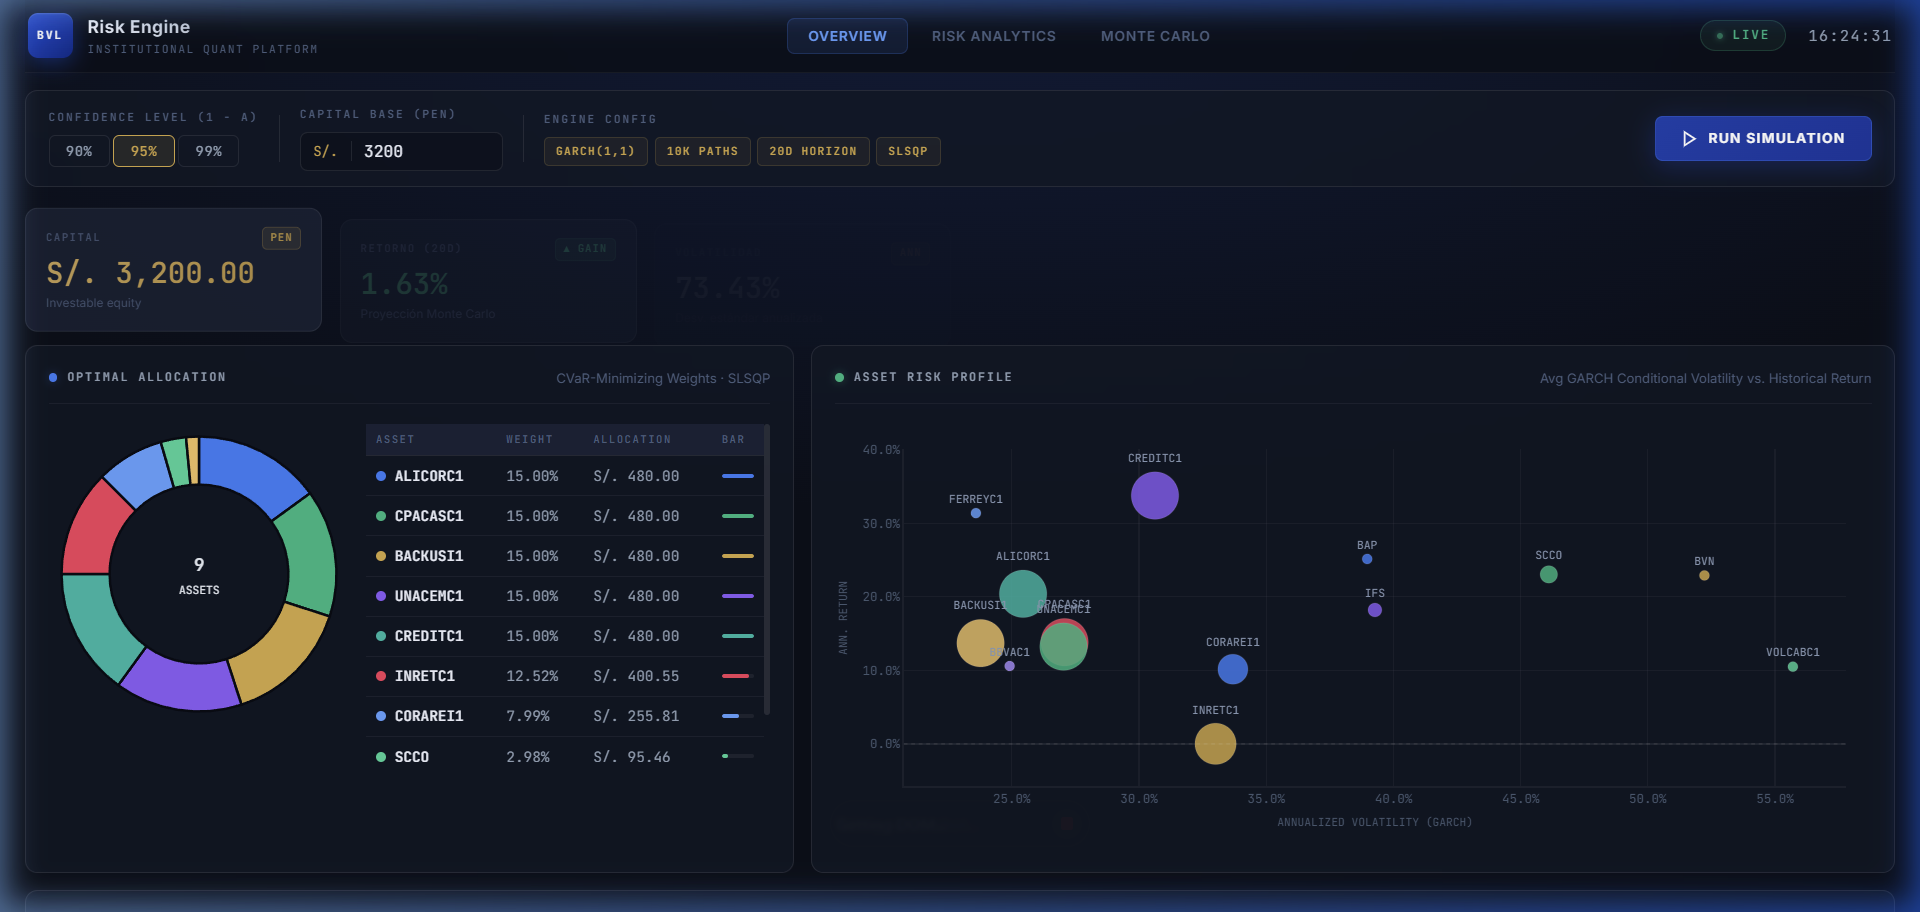
\includegraphics[width=0.9\textwidth]{figures/dashboard.png}
    \caption{Vista general del Dashboard: KPIs, asignación de activos y distribución del Monte Carlo.}
    \label{fig:dashboard}
\end{figure}

\begin{figure}[h!]
    \centering
    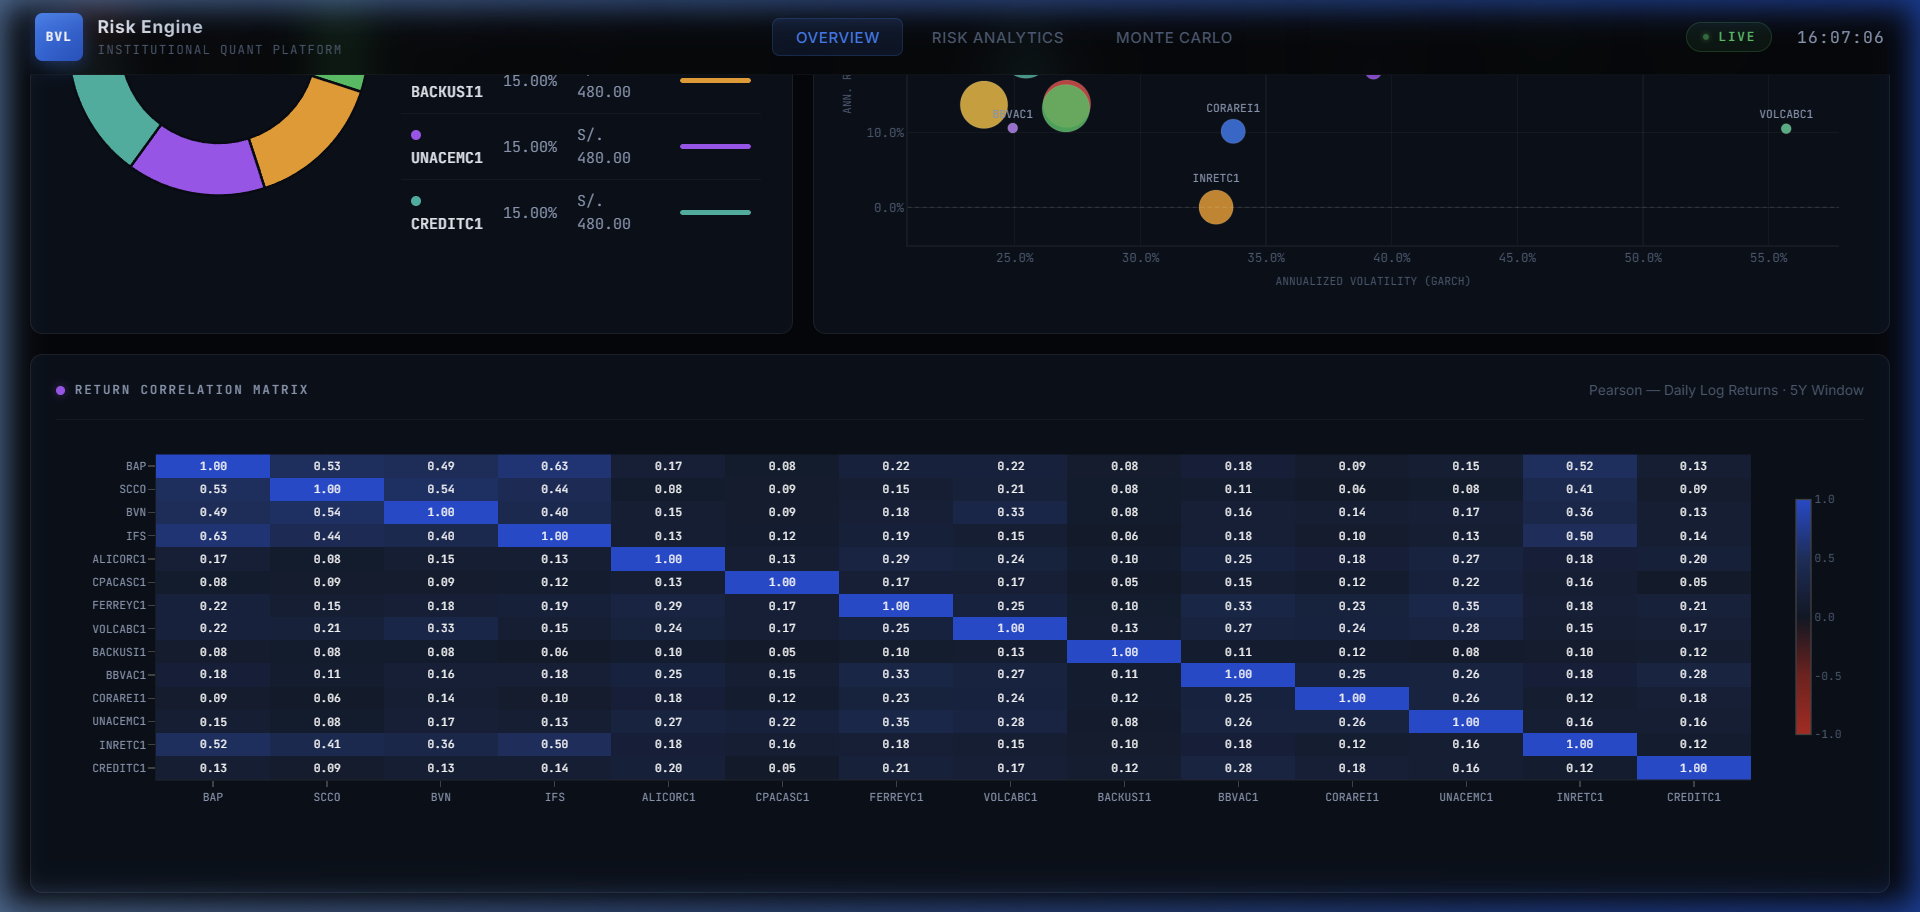
\includegraphics[width=0.9\textwidth]{figures/monte_carlo.png}
    \caption{Proyección de 10,000 trayectorias de Monte Carlo con técnica de Block Bootstrap para preservar la memoria del mercado (volatility clustering).}
    \label{fig:monte_carlo}
\end{figure}

\begin{figure}[h!]
    \centering
    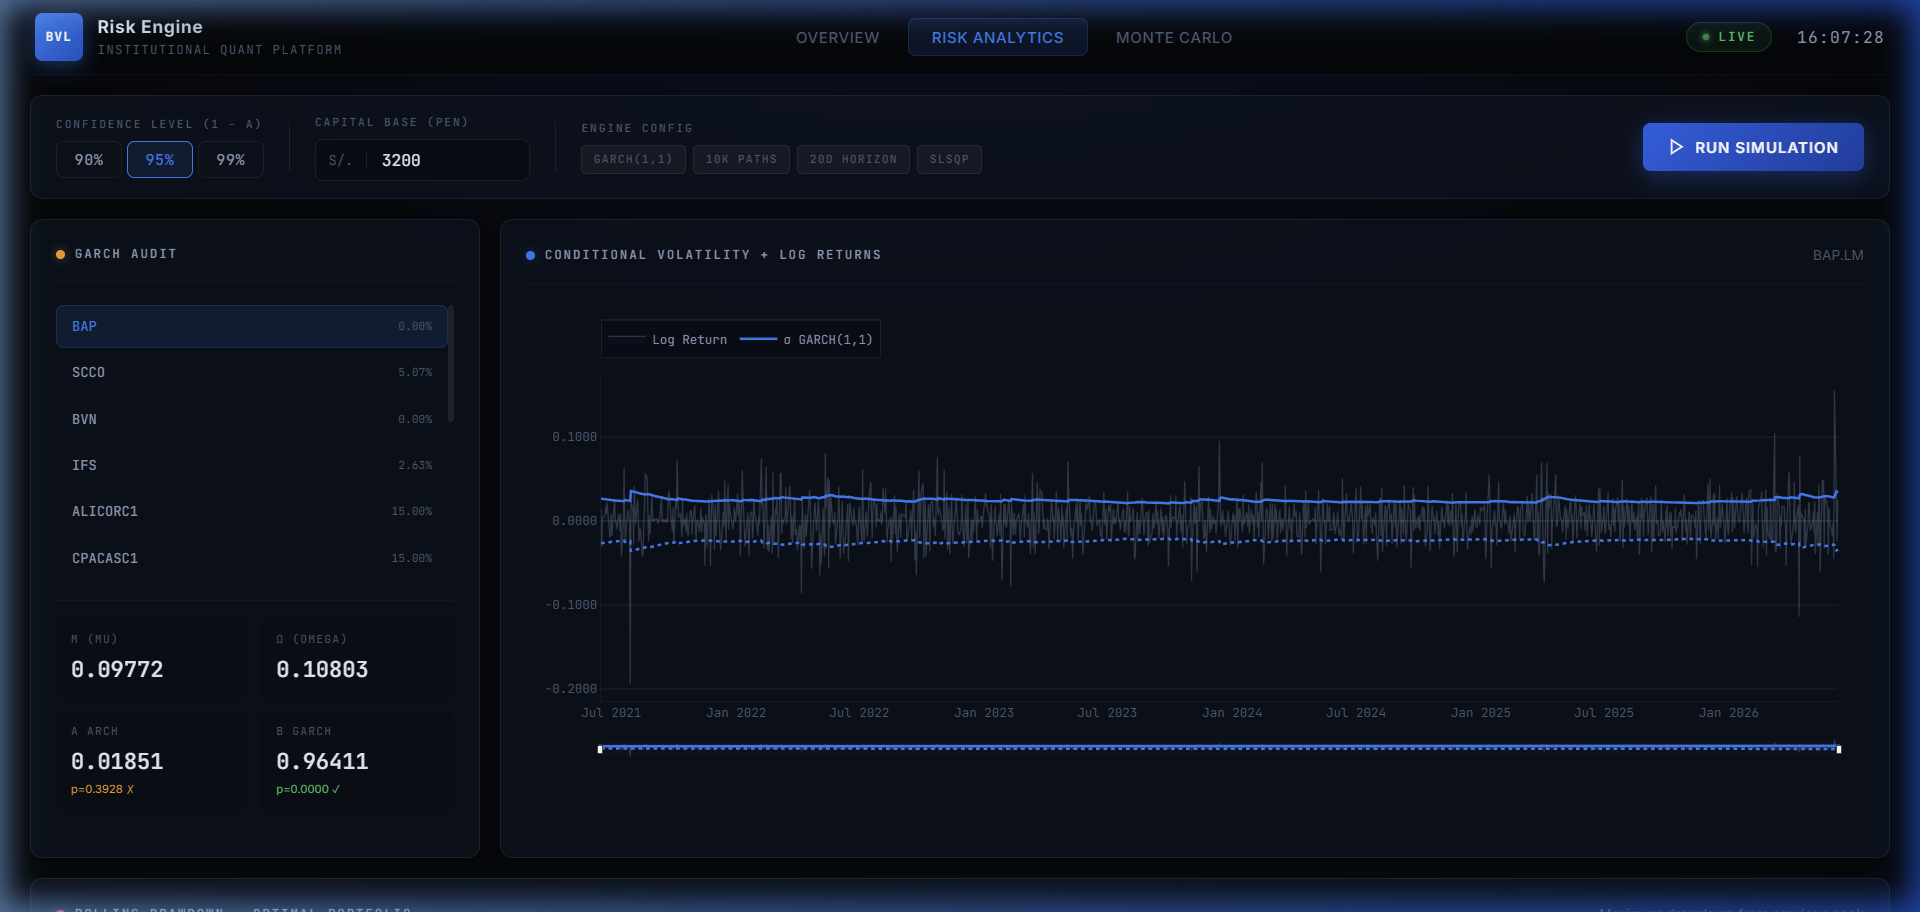
\includegraphics[width=0.9\textwidth]{figures/risk_analytics.png}
    \caption{Auditoría GARCH: Selección dinámica de distribución y proyección de volatilidad condicional.}
    \label{fig:risk_analytics}
\end{figure}

\section{Utilidad para Inversores e Instituciones}

El grado institucional de este motor cuantitativo aporta un valor crítico en tres frentes:

\begin{enumerate}
    \item \textbf{Gestión de Riesgos (Risk Management):} Las áreas de riesgo de un banco pueden utilizar el motor para estresar el portafolio (Stress Testing) de sus clientes, estimando con alta confianza científica el tamaño de los "drawdowns" potenciales.
    \item \textbf{Gestión de Activos (Asset Management):} Los Portfolio Managers dejan de guiarse por intuición o modelos desfasados de M-V (Media-Varianza). Al minimizar el CVaR, aseguran que los retornos ajustados por riesgo extremo se mantengan dentro de los parámetros del mandato institucional.
    \item \textbf{Auditoría y Compliance:} El módulo \textit{GARCH Audit} transparenta totalmente los coeficientes $(\alpha, \beta, \omega, \nu, \lambda)$ utilizados en el motor de riesgo interno, facilitando explicaciones ante reguladores sobre cómo se calculan las reservas de capital frente a riesgos de mercado.
\end{enumerate}

\section{Conclusión}
El Motor Cuantitativo BVL consolida las técnicas de frontera del análisis cuantitativo (Block Bootstrap, Distribuciones Skewed-t dinámicas, Optimización CVaR) en un producto tecnológico ágil y visual. Constituye una herramienta fundacional robusta para la asignación de activos en la región latinoamericana.

\end{document}
